\documentclass[11pt, oneside]{article}   	% use "amsart" instead of "article" for AMSLaTeX format
\usepackage[utf8]{inputenc}

\usepackage{lmodern}
\usepackage[T2A]{fontenc}
\usepackage{cmbright}
\usepackage[russian]{babel}
%\usetheme{Darmstadt}


\usepackage{amsmath}
\usepackage{amsfonts}
\usepackage{bm}
\usepackage{graphicx}
% Использовать полужирное начертание для векторов
\let\vec=\mathbf

\DeclareMathOperator{\mathspan}{span}
\DeclareMathOperator{\mathdim}{dim}
\DeclareMathOperator{\rank}{rank}
\DeclareMathOperator{\diag}{diag}

\begin{document}
	\author{Е. Ларин, Ф. Ежов, И. Кононыхин }
	\title{Обучение с учителем. Классификация. Дискриминантный анализ. }
%	\subtitle{Санкт-Петербургский государственный университет 
%		
%		Прикладная математика и информатика
%		
%		Вычислительная стохастика и статистические модели
%	}
	\date{}
	%\subject{Семинар по статистическому и машинному обучению}


		\maketitle 

		\section{Обучение с учителем}
		Рассмотрим задачу обучения с учителем, частным случаем которой являются задачи классификации и регрессии.

		Алгоритм в общем виде имеет вид:
		\begin{itemize}
			\item \textit{Вход}: $\bm{X}$ --- выборка $\bm{\xi}$, случайной величины признаков, $\bm{y}$ --- выборка $\eta$, случайной величны <<ответов>> (принадлежность к классу для классификации, либо значение функции для регрессии). Предполагаем, что существует неизвестное отображение $y^*: \bm{\xi} \to \eta$  (гипотеза непрерывности или компактности)
			
			\item \textit{Задача}: По $\bm{X}$ и $\bm{y}$ найти такое отображение $\hat{y}^*: \bm{\xi} \to \eta$, которое приблизит отображение  $y^*$. 
			
			\item \textit{Оценка}: Функция потерь $\mathfrak{L}(y^*(x), \hat{y}^*(x))$. Здесь $x$ --- реализация $\bm{\xi}$
		\end{itemize}

		\section{Классификация}
		Перейдём к задаче классификации. Как и в задаче регрессии, данные должны происходить из некоторой генеральной совокупности. 
		
		Будем рассматривать выборку признаков и ответов~\ref{1}
		\begin{equation}
			\bm{X} \in \mathbb{R}^{n\times p}, \;\;\mathbf{y}\in \mathbb{A}^n.
			\label{1}
		\end{equation}
		
		Отметим, что множество $\mathbb{A}^n$ не является непрерывным. Размерность этого множества $k\times n$, где $k$ --- количество возможных классов.
		
		Для обоснования применения методов классификации используется \textbf{\textit{гипотеза компактности}}:
		
		<<Близкие>> объекты, как правило, принадлежат одному классу.
		\newline



		\subsection{Классификация: вероятностная постановка}
		Поставим задачу классификации в терминах генеральных случайный величин.
		
		\textit{Дано:}
		\begin{itemize}
			\item $\bm{\xi} \in \mathbb{R}^p$ --- вектор признаков
			\item $\eta \in \mathbb{A}$ --- классовая принадлежность
		\end{itemize}
	
		Предположение об их зависимости можно записать в виде \ref{2}.
		\begin{equation}
			\eta = \Phi(\bm{\xi})
			\label{2}
		\end{equation}
		
		\textit{Задача:} найти $\Phi$
		
		При переходе к выборкам, случайная величина признаков $\bm{\xi}$ заменяется на матрицу наблюдений $\bm{X}$, а случайная величина ответов $\eta$ --- на вектор классовой принадлежности $\bm{y}$.
		
		Предположение принимает вид \ref{3}.
		\begin{equation}
			y_i = \Phi(\bm{x}_i),\;\;\; i = 1, \ldots, n
			\label{3}
		\end{equation}
		

		\subsection{Классификация: оценка качества}
		\label{metrics}
		\begin{figure}
			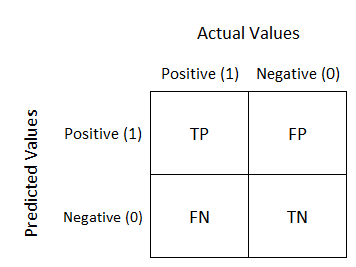
\includegraphics[width=0.3\linewidth]{imgs/conf_matrix}
			\label{conf_matrix}
			
		\end{figure}
	    На основе матрицы ошибок~\ref{conf_matrix} есть большое количество разных метрик. Приведём некоторые из них: 
	    \begin{itemize}
	    	\item\textit{accuracy} = ${TP + TN}\over{TP+TN+FP+FN}$, 
	    	\item\textit{recall} = ${TP}\over{TP+FP}$, 
	    	\item\textit{precision} = ${TP + TN}\over{TP+FN}$, 
	    	\item $F_\beta = (1-\beta^2) {{precision \times recall}\over{(\beta^2 \times precision) + recall}}$, 
	    	\item\textit{ROC--AUC}
	    \end{itemize}


		\subsection{Классификация: этапы обучения модели}
		\begin{itemize}
			\item Выбор модели (класс рассматриваемых $\Phi$ из \ref{3}).
					 Здесь будут рассмотрены модели LDA и QDA. 
			\item Выбор функции потерь.
					 Чаще всего это $\sum_{i=1}^{n}(y_i \neq \widehat{y}_i)$.
			\item Выбор метода обучения.
			 		Выбор способа подбора параметров для минимизации функции потерь на обучающем множестве.
			\item Выбор метода проверки.
			 		Выбор оценки качества модели, например, с помощью метрик из раздела~\ref{metrics}.
		\end{itemize}

%		\subsection{Классификация: задача оптимизации}
%		\begin{itemize}
%			\item $\hat{\beta}$ --- параметры модели
%			\item $\bm{\Phi}(\bm{x}, \beta)$ --- функционал классификации
%			\item $\mathfrak{L}(\bm{\Phi}(\bm{x}, \beta), \bm{y})$ --- функция потерь (метрика)
%		\end{itemize}
%		\begin{block}{}
%			$$\hat{\beta} = \arg\min_{\beta} \mathfrak{L}(\bm{\Phi}(\bm{x}, \beta), \bm{y})$$
%		\end{block}

		\subsection{Классификация: общий подход к решению}
		Как построить функционал $\Phi$?
		
		
		Общий подход --- построить набор классифицирующих функций $f_i$, $i = 1, \ldots, K$. Каждая функция $f_i(\bm{x})$ показывает меру принадлежности $\bm{x}$ классу $i$. 
		
		Таким образом, решение о принадлежности классу принимается при обнаружении классифицирующей функции с наибольшим значением:
		\begin{equation}
			\Phi(\bm{x}) = \arg\max_i(f_i(\bm{x})).
			\label{4}
		\end{equation}

		\section{Дискриминантный анализ}
		Примем за функции $f_i$ из \ref{4} оценку вероятности принадлежности к $i$-му классу.
		
		$$\Phi(\bm{x}) = \arg\max_i (P(C_i|\bm{x})).$$
		
		$C_i$ ---  класс, состоящий из одного события: $\bm{x}$ принадлежит $i$-му классу.

		Если известны априорные вероятности получения $i$-го класса ($\pi_i$), применим формулу Байеса
		
		$$P(C_i|\bm{x}) = {{\pi_i P(\bm{x}|C_i)}\over{\sum_{j=1}^{K} \pi_j P(\bm{x}|C_j)}}.$$
		 
		 Отбросим знаменатель
		
		$$f_i = P(C_i|\bm{x}) = \pi_i P(\bm{x}|C_i).$$
 
		\subsection{LDA}
		Предположим, что искомые классы имеют многомерное нормальное распределение с равными дисперсиями.
		
		Запишем это в виде формулы:

		$$\mathtt{P}(\bm{\xi}|\eta = A_i) = \mathtt{N}(\bm{\mu}_i, \bm{\Sigma})$$
		
		Построим классифицирующие функции:
		$$f_i(\bm{x}) = {{\pi_i}\over{(2\pi)^{p/2}|\bm{\Sigma}|^{1/2}}}exp\left(-{{1}\over{2}}(\bm{x} - \bm{\mu}_i)\bm{\Sigma}^{-1}(\bm{x} - \bm{\mu}_i)^\mathtt{T}\right)$$
		
		Немного упростим (подробнее было изложено в одном из предыдущих курсов):
		\begin{equation}
			h_i(\bm{x}) = -0.5 \bm{\mu}_i\bm{\Sigma}^{-1}\bm{\mu}_i^\mathtt{T} + \bm{\mu}_i\bm{\Sigma}^{-1}\bm{x} + \log\pi_i
		\label{lda}
		\end{equation}
		Функции~\ref{lda} применяются при классификации данным методом.


		\subsection{QDA}
		
		Предположим, что искомые классы имеют многомерное нормальное распределение с различными дисперсиями.
		
		Запишем это в виде формулы:
		$$\mathtt{P}(\bm{\xi}|\eta = A_i) = \mathtt{N}(\bm{\mu}_i, \bm{\Sigma}_i)$$
		
		Построим классифицирующие функции:
		$$f_i(\bm{x}) = {{\pi_i}\over{(2\pi)^{p/2}|\bm{\Sigma}_i|^{1/2}}}exp\left(-{{1}\over{2}}(\bm{x} - \bm{\mu}_i)\bm{\Sigma}_i^{-1}(\bm{x} - \bm{\mu}_i)^\mathtt{T}\right)$$
		
		Немного упростим (подробнее было изложено в одном из предыдущих курсов):
		\begin{equation}
			g_i(\bm{x}) = -0.5 (\bm{x} - \bm{\mu}_i)\bm{\Sigma}^{-1}(\bm{x} - \bm{\mu}_i)^\mathtt{T} - 0.5\log|\bm{\Sigma}_i| + \log\pi_i
			\label{qda}
		\end{equation}
		
		Функции~\ref{qda} применяются при классификации данным методом.

%		\section{Классификация и регрессия}
%		
%		Сравним модели линейной регрессии и бинарной классификации.
%		\subsection{Регрессия}
%		Обучающая выборка: $\bm{X} \in \mathbb{R}^{n \times p}, \;\;\mathbf{y}\in \mathbb{R}^n$.
%		
%		\begin{enumerate}
%			\item Модель регрессии:
%			$$ \hat{\bm{y}} = \bm{\Phi}(\bm{x}, \beta) = \langle \bm{x}, \beta \rangle = \sum\limits_{j=1}^{p} \beta_j x_j , \; \beta \in \mathbb{R}^p$$
%			
%			\item Функция потерь:
%			$$ \mathfrak{L}(\hat{\bm{y}}, \bm{y}) = (\hat{\bm{y}} - \bm{y})^2$$
%			
%			
%			\item Метод обучения --- метод наименьших квадратов:
%			$$ Q(\beta) = \sum\limits_{i = 1}^{n} (\bm{\Phi}(\bm{x}_i, \beta) - \bm{y}_i)^2 \rightarrow \min\limits_{\beta} $$
%			
%		\end{enumerate}
%
%		\subsection{Классификация}
%		Обучающая выборка: $\bm{X} \in \mathbb{R}^{n\times p}, \;\; y \in \{-1, 1\}$.
%		
%		\begin{enumerate}
%			\item Модель классификации:
%			$$ \hat{y} = \bm{\Phi}(\bm{x}, \beta) = sign \langle \bm{x}, \beta \rangle = sign \sum\limits_{j=1}^{p} \beta_j x_j , \; \beta \in \mathbb{R}^p$$
%			
%			\item Функция потерь:
%			$$ \mathfrak{L}(\hat{y}, y) = [\hat{y} y < 0] = [ \langle \bm{x}, \beta \rangle y < 0 ] \leq \hat{\mathfrak{L}}( \langle \bm{x}, \beta \rangle y) $$
%			
%			
%			\item Метод обучения --- минимизация эмпирического риска:
%			$$ Q(\beta) = \sum\limits_{i = 1}^{n} [\langle \bm{x}_i, \beta \rangle y_i < 0] \leq \sum\limits_{i = 1}^{n} \hat{\mathfrak{L}}( \langle \bm{x}_i, \beta \rangle y_i)  \rightarrow \min\limits_{\beta} $$
%			
%		\end{enumerate}
%
%		\section{Отступы}
%		
%		$\bm{\Phi}(\bm{x}, \beta) = sign  (g(\bm{x}, \beta))$ --- разделяющий классификатор,\\
%		$g(\bm{x}, \beta)$ --- разделяющая функция,\\
%		$g(\bm{x}, \beta) = 0$ --- уравнение разделяющей поверхности.\\
%		
%		\bigskip
%		
%		$M_i(\beta) = g(\bm{x}_i, \beta) y_i$ --- отступ объекта $\bm{x}_i$. \\
%		Если $M_i(\beta) < 0$, тогда алгоритм ошибается на $\bm{x}_i$.
%	
%
%		\section{Отступы}
%		\begin{figure}
%			\centering
%			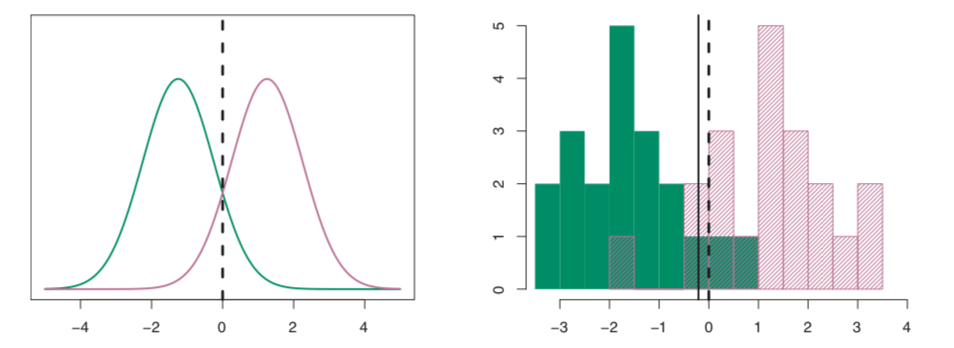
\includegraphics[width=0.7\linewidth]{imgs/margins}
%			
%
%		\end{figure}


	
\end{document}